\section*{Question 3}
\fakesection{3}

This problem repeats the polyphase interpolator of Question 2, but adds the additional task of frequency shifting the interpolated signal by heterodyning with a 10 kHz carrier. This is easily achieved with a signal extra step. After zero-padding and reshaping the filter coefficients into a matrix of $L$ rows, where $L$ is the upsampling factor, we multiply each row by
\begin{align}
    c(n) = \cos(2\pi nk/M),\ n = 0..L-1
\end{align}
where $n$ is the row index and $k$ is a constant which determines the shift:
\begin{align}
    k = L \cdot \frac{f_c}{f_s}
\end{align}
Here, $f_c$ is the carrier frequency, 10 kHz, and $f_s$ is the frequency after upsampling, 40 kHz. Then, applying the filter to the signal using the same method described for Question 2, the input signal is upsampled, filtered and frequency shifted.

\begin{figure}[ht]
    \centering
    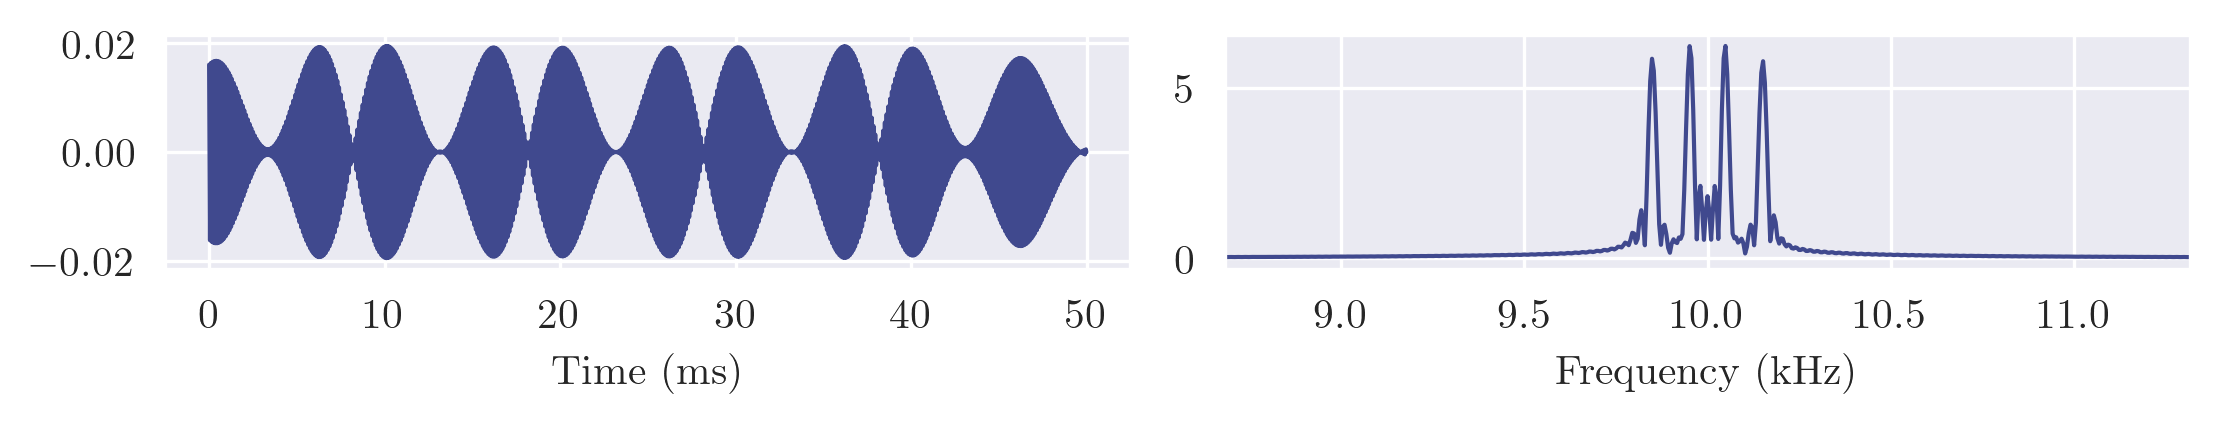
\includegraphics[width=0.8\textwidth]{images/q3_heterodyne.png}
    \caption{Simultaneous heterodyning with 10 kHz carrier by polyphase interpolator}
    \label{fig:q3_heterodyne}
\end{figure}

Performing 10,000 trials for comparison with the timing results of Question 2, we find the average time per trial is 0.801 ms. This is actually equal to the timing without heterodyning (to the presented precision), though typically we would expect some variance. Hence, we have achieved our aim of heterodyning without incurring any significant additional computation.
